% !TeX encoding = UTF-8

\chapter{IMPLEMENTAÇÃO}\label{ch:implementacao}

Neste capítulo serão abordadas questões do planejamento e da implementação do sistema de reconhecimento de faces em vídeo. Primeiramente, os requisitos do sistemas serão analisados e descritos, seguidos da modelagem destes requisitos em forma de fluxograma, seguidos da modelagem das classes que serão criadas por meio dos diagramas descritos na \autoref{subsec:uml}, e por fim, as questõs de configuração do ambiente de desenvolvimento e a implementação efetiva do código. Todo este processo é feito seguindo conceitos da metodologia ágil XP, descrita na \autoref{subsec:devagil}.

\section{Análise de Requisitos}\label{sec:analiserec}
Para que se possa iniciar o planejamento da implementação do sistema aqui proposto por meio de diagramação, deve-se colher os requisitos necessários para o funcionamento do sistema. Ou seja, analisar o problema descrevendo entredas e saidas de dados, todas as situações e seus fluxos de informações. Sendo assim lista-se por ordem de execução os requisitos que atendem à proposta do sistema, discriminados por \textbf{entrada}, \textbf{processamento} e \textbf{saída} de dados ou informações:

\begin{enumerate}
	\item \textbf{entrada:} uma câmera do tipo \textit{webcam} descrita na \autoref{sec: tec-ferramenta} deve estar filmando uma área com iluminação controlada, produzindo o fluxo de \textit{frames} e disponibilizando em formado digital para o sistema;
	
	\item \textbf{processamento:} o sistema adquire controle do fluxo de \textit{frames} da \textit{webcam}, manipulando-o para que se possa ser exibido na tela do microcomputador e realiza a detecção de uma face, em tempo real, utilizando o algoritmo descrito na \autoref{subsubsec:violajones} com os materiais contemplados na \autoref{subsec:bib_opencv};
	
	\item \textbf{saída:} o sistema exibe, em tempo real, o fluxo de \textit{frames} processado como define o item acima, na tela do microcoputador. Ao mesmo tempo, caso seja detectada uma face, o sistema deverá desenhar um retângulo em volta da face detectada neste fluxo de \textit{frames}, ativando um campo para que o usuário possa entrar com uma identificação da face detectada;
	
	\item \textbf{entrada:} o usuário entra com uma identificação da face detectada, caso haja, em um campo disponibilidado pelo sistema (por exemplo, um nome);
	
	\item \textbf{processamento:} o sistema inicia o processo de treinamento da face definido na \autoref{sec:recog_faces}, criando um \textit{eigenspace}, e no momento seguinte à criação deste "plano cartesiado", o sistema já deve realizar o processo de reconhecimento descrito na \autoref{subsec:reconhecimento};
	
	\item \textbf{saída:} caso seja reconhecida uma face no fluxo de \textit{frames}, tal como descrito no item acima, o sistema deve exibir a identificação introduzida pelo usuário com define o item "4";
\end{enumerate}



\section{Diagrama de Fluxo de Dados}\label{sec:fluxorec}

O diagrama de fluxo é uma técnica que apresenta de forma gráfica, sequêncial, as atividades de um processo para facilitar a visualização de suas etapas \cite{fluxogramalivro}.

Na elaboração deste diagrama, considera-se que os requisitos listados na seção 4.1"ocorrem em tempo-real. Sendo assim, todas as tarefas necessárias para atender os requisitos devem ser executados em um \textit{loop}, exceto para o requisito de entrada identificação da face (item 4) e o requisito de treinamento (item 5, de processamento), que ocorrerão apenas caso o usuário introduza a informação.

A fluxograma da \autoref{fig:fluxoreq} dispõe os requisitos e o diagrama de fluxo de dados:


\begin{figure}[h]
	\centering
	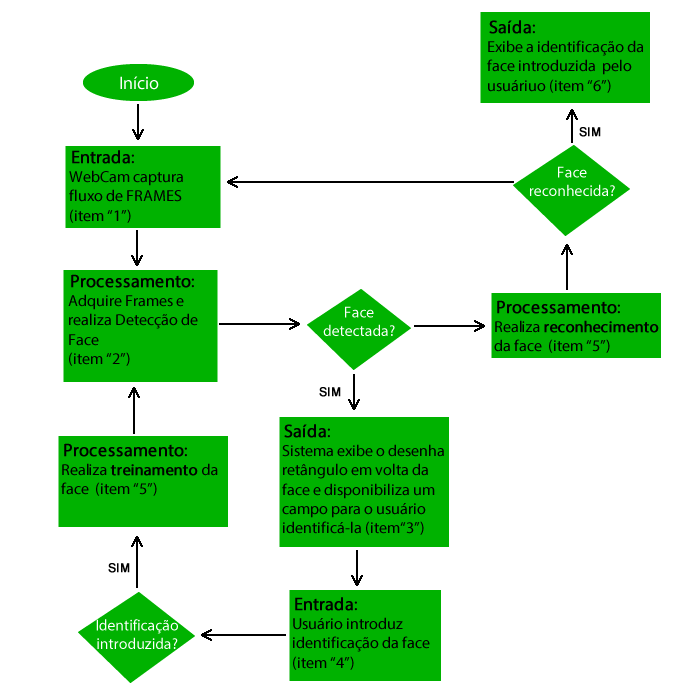
\includegraphics[width=.8\textwidth]{fluxo}
	\caption{Fluxograma representando os requisitos que devem ser atendidos.}
	\fonte{Elaborado pelo autor.}
	\label{fig:fluxoreq}
\end{figure}


\section{Diagrama de Classes}\label{sec:diagclasses}
Nesta seção, as classes que serão criadas para implementação do sistema aqui proposto serão apresentadas em forma de diagrama de classes e posteriormente descritas. A \autoref{} ilustra tal diagrama:









%\codigoPython
%\lstinputlisting[language=Python, label=coleta-script, caption=\textit{Script} coletar-hashtags.py]{src/coletar-hashtags.py}
